\documentclass[a4paper, 12pt]{article}

\def \patha {} %Pfad zu den Dateien Preamble.tex, Commands.tex, Erwartungsbild.tex

\input{\patha/Preamble.tex}

\onehalfspacing

\newcommand{\KopfzeileBlank}{true}
\newcommand{\FACH}{Informatik}
\newcommand{\KLASSE}{5}
\newcommand{\DATUM}{\rule[0ex]{2cm}{1pt}}
%% Über den jeweiligen Typ wird bei Klassenarbeit und Leistungskontrolle das Erwartungsbild und der Notenspiegel als anhängende Seite kompiliert. Der Befehl \aufgabe besitzt beim Typ Arbeitsblatt einen Parameter für die Aufgabenstellung. Bei den Typen Klassenarbeit und Leistungskontrolle kommen noch zwei weitere Parameter für die Punktzahl und das Erwartungsbild hinzu.
%\newcommand{\TYP}{Arbeitsblatt}
%\newcommand{\TYP}{Klassenarbeit}
\newcommand{\TYP}{Leistungskontrolle}
\newcommand{\EINHEIT}{Bilder und Grafiken gestalten}
\newcommand{\THEMA}{Bilder und Grafiken gestalten}
\newcommand{\LEHRER}{N.N.}
\newcommand{\TIME}{25 Min.}
\newcommand{\NTA}{Vereinfachte Aufgabenstellungen und Zeitverlängerung}
%% Dieser "Switch" bewirkt, dass für Lückentexte die Lösung angezeigt oder ausgeblendet wird. Aktuell werden die Lücken jedoch noch nicht berücksichtigt. Vielleicht gibt es auch eine bessere Lösung für diesen "Switch"...
%\newcommand{\LOSUNG}{true}
\newcommand{\LOSUNG}{false}

%\input
\input{\patha/Commands.tex}

\begin{document}

\Large
\TITEL

\aufgabe{Nenne das Englische Wort für Bildpunkt}{1}{Pixel}
\liniert{1}

\aufgabe{Ein Pixel ist aus drei Subpixeln aufgebaut. Kreuze die Farben an, aus denen die Subpixel bestehen.}{3}{0,5 Punkte je richtiges Kreuz und je freigelassenes Kästchen}
\begin{tasks}(3)
	\task \Square\ Gelb
	\task \Square\ Rot
	\task \Square\ Weiß
	\task \Square\ Grün
	\task \Square\ Blau
	\task \Square\ Orange
\end{tasks}


\aufgabe{Entscheide dich, ob die Eigenschaften zu einer Vektor- oder eine Pixelgrafik gehören.}{4}{1 Punkt je richtiges Kreuz:\begin{center}
\begin{tabular}{|l|c|r|}
	\hline
	Pixelgrafik & & Vektorgrafik \\\hline
	 X& Verpixelt beim vergrößern&\\\hline
	 X& Jeder Pixel kann bearbeitet werden&\\\hline
	 & Ist eine Beschreibung für den Computer&X\\\hline
	 & Kann beliebig vergrößert werden&X\\\hline
\end{tabular}
\end{center}}
\begin{center}
\begin{tabular}{|l|c|r|}
	\hline
	Pixelgrafik & & Vektorgrafik \\\hline
	 & Verpixelt beim vergrößern&\\\hline
	 & Jeder Pixel kann bearbeitet werden&\\\hline
	 & Ist eine Beschreibung für den Computer&\\\hline
	 & Kann beliebig vergrößert werden&\\\hline
\end{tabular}
\end{center}


\aufgabe{Gib die Auflösung der beiden Bilder an. Begründe, welches Bild die höhere Auflösung hat.}{3}{Hund\_1: 800x600 Pixel (1P.), Hund\_2: 600x800 Pixel (1P.), Begründung: Die Bilder haben die gleiche Auflösung (1P.).}
\begin{minipage}{0.49\linewidth}
	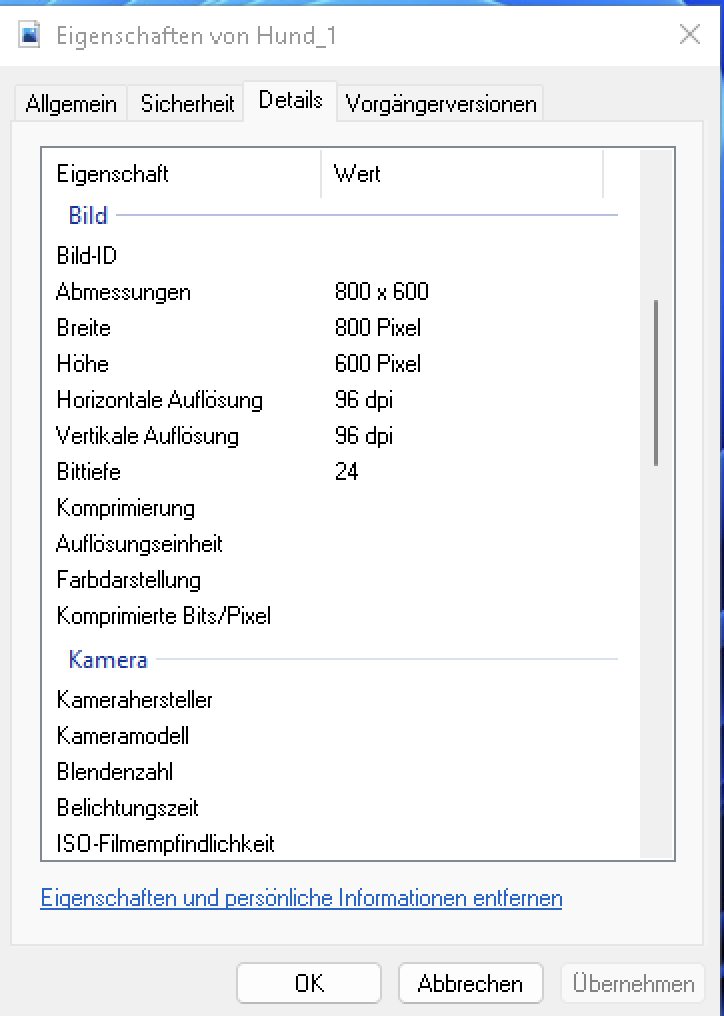
\includegraphics[scale=0.7]{Hund_1.png}
\end{minipage}
\begin{minipage}{0.49\linewidth}
	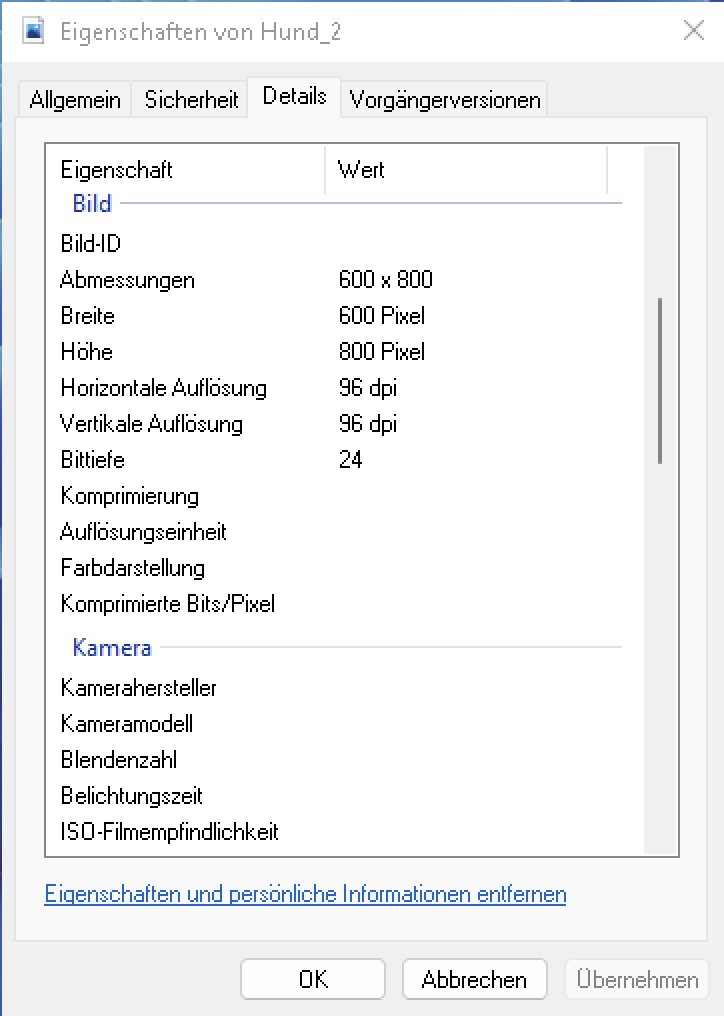
\includegraphics[scale=0.7]{Hund_2.png}
\end{minipage}
\vspace{1cm}
\begin{LKtext}
	Auflösung des Bildes "Hund\_1": \lk{800} x \lk{800} Pixel.
	
	Auflösung des Bildes "Hund\_2": \lk{800} x \lk{800} Pixel.
\end{LKtext}

\subsubsection*{Begründung:}
\liniert{3}

%\input
\label{LastPage}
\normalsize
\ifthenelse{\equal{\TYP}{Klassenarbeit}}{
\input{\patha/Erwartungsbild.tex}}
{}
\ifthenelse{\equal{\TYP}{Leistungskontrolle}}{
\input{\patha/Erwartungsbild.tex}}
{}


\end{document}